% !TeX root=main.tex

\chapter{ارزیابی روش پیشنهادی} \label{ch:eval}
\thispagestyle{empty}


\section{مقدمه}
\paragraph{}{
    در این فصل برای بررسی عملکرد روش پیشنهادی در فصل قبل، سیستم مورد نظر به طور کامل پیاده‌سازی
    شده و بر روی یک مجموعه‌داده‌ی شناخته‌شده اجرا شده است.
    برای ارزیابی روش پیشنهادی روش‌های متفاوتی ارائه شده است. 

    برای انتخاب رویکرد مناسب ارزیابی از میان خیل عظیمی از روش‌های شناخته‌شده
    عوامل متعددی مورد بررسی قرار می‌گیرد و با توجه به آن‌ها یک یا چند روش انتخاب می‌شود.
    مهم‌ترین عامل ساختار و جنس داده‌های خروجی مدل و همچنین جنس داده‌های ارزیابی است. باتوجه به مدل و مجموعه
    داده‌ مورد استفاده، در این پژوهش نیاز به معیارهای ارزیابی برای مقایسه جملات داریم. 
    از آنجایی که این روش، روشی نو است برای اثبات درستی آن از معیار‌های ارزیابی متفاوتی استفاده کردیم 
    که به طور کلی در دو بخش دسته‌بندی می‌شود. 
}

\section{
    معیارهای برپایه شباهت نحوی
}
\label{sec:wordbased}
\paragraph{}{
    معیارهای برپایه شباهت نحوی به یکسان بودن توکن‌ها در
    یک جمله تمرکز دارد. به عبارتی براساس تعداد توکن‌های 
    انتخابی و برابری آن‌ها امتیازی بین دو جمله در نظر گرفته
    شده که نشانگر میزان شباهت دو جمله به یکدیگر است. 
    در این پژوهش از معیارهای 
    BLEU \cite{papineni2002bleu}،
    Rouge \cite{lin2004rouge}،
    و
    METEOR \cite{banerjee2005meteor}
    به عنوان معیارهای شباهت بر پایه توکن‌ها استفاده‌ شده است.
    این معیارها معمولا برای ترجمه‌های ماشینی استفاده می‌شوند و از آنجایی
    که هدف مقایسه دو جمله پاسخ و جمله مرجع است 
    استفاده از این معیارها برای سنجش سیستم راه حل مناسبی است.

}

\section{
  معیارهای برپایه بردارهای تعبیه
} \label{sec:embeddingbased}
\paragraph{}{
    در این معیارها با بهره‌برداری از بردارهای تعبیه
    \footnote{\lr{Embedding vectors}}
    به محاسبه شباهت بین جملات پرداخته می‌شود. 
    در این پژوهش از دو معیار
    BERTScore \cite{zhang2019bertscore}
    و 
    \lr{Average Score}
    به عنوان معیارهای بردار تعبیه استفاده شده است.
}

\subsection{
  معیار BERTScore \cite{zhang2019bertscore}
} \label{subsec:BERTScore}
% \vspace*{10pt}
\paragraph{}{
    BERTScore 
    یک معیار ارزیابی خودکار است که برای ارزیابی 
    سیستم‌های تولید متن استفاده می‌شود.
    برخلاف روش‌های رایج موجود که شباهت 
    نحوی توکن‌ها را محاسبه می‌کنند، 
    BERTScore 
    بر محاسبه شباهت معنایی بین توکن‌های مرجع و
    توکن‌های پیش‌بینی شده تمرکز دارد. 
    نویسنده مقاله آن را بر روی ترجمه‌های ماشینی و 
    وظایف توضیح تصاویر آزمایش کرد و 
    دریافت که با قضاوت های انسانی ارتباط بهتری دارد.

    از مزایای این معیار نسبت به مقایسه نحوی می‌توان به عدم محاسبه 
    توکن‌های هم‌معنی در نظر گرفت. برای مثال معیارهای برمبنای شباهت نحوی، 
    درصورت مغایرت توکن‌ها هیچ امتیازی در نظر نمی‌گیرند در حالی که
    BERTScore
    به نزدیکی معانی کلمات توجه می‌کند.
}

\subsection{
    معیار 
    Score Average
} \label{subsec:average-score}
    % \vspace*{10pt}
\paragraph{}{
    برای محاسبه این معیار، در ابتدا یک میانگین از بردارهای تعبیه جملات گرفته 
    و سپس با استفاده از تابع شباهت کسینوسی میزان شباهت بین جملات مرجع و جملات
    پیش‌بینی شده محاسبه می‌شود.
    (معادله \ref{eq:avg-score-sim})
    \begin{equation}
        \label{eq:avg-score}
        Score(s = [t_1, t_2, ..., t_T]) = \frac{1}{T}\sum_{i=0}^{T}{Embedding(t_i)}
    \end{equation}

    \begin{equation}
        \label{eq:avg-score-sim}
        sim(s_1, s_2) = \frac{\vec{Score(s_1)}.\vec{Score(s_2)}}{||Score(s_1)||\times||Score(s_2)||} 
    \end{equation}
}


\section{
  مجموعه‌داده‌ی مورد استفاده
 }
 \label{sec:dset}
\paragraph{}{
    در بخش 
    \ref{sec:vqa_datasets}
    به معرفی بخش اعظمی از مجموعه‌ داده‌های موجود
    در پرسش‌وپاسخ تصویری پرداخته‌شد. با این حال اگر
    به این مجموعه‌ داده‌ها با دید عمیق تری بنگریم متوجه این
    موضوع می‌شویم که در هیج‌کدام از این مجموعه‌ها پاسخ‌ها
    به صورت جمله کامل نیستند، به عبارتی برای 
    حل آن‌ها استفاده از دسته‌بندی کافی است. برای ارزیابی دقیق
    سیستم پیشنهادی نیازمندی مجموعه داده‌ای است که پاسخ‌های 
    پرسش‌ها به صورت جمله باشد. 
    مجموعه داده 
    \lr{Full Sentence Visual Question Asnwering (FSVQA)}
    \cite{shin2016color}
    این خاصیت را دارد و بهترین گزینه برای استفاده به عنوان 
    مجموعه داده ارزابی است. 

    مجموعه داده FSVQA 
    شامل یک تصویر و یک پرسش مربوط به آن است 
    و جمله یه صورت پاسخ آن پرسش به عنوان
    هدف در نظر گرفته شده است. 
    این پاسخ‌ها از دو مجموعه داده 
    VQA \cite{VQA}
    و 
    MSCOCO \cite{caesar2018coco}
    و بر اساس قوانین زبان 
    انگلیسی به صورت خودکار تولید شده‌اند. 
    توجه به این نکته حائز اهمیت است که تولید جملات از 
    این روش امکان 
    ایجاد اشکالاتی را در مجموعه داده بوجود می‌آورد 
    و مدل‌ها نیز قادر به یادگیری الگوی پاسخ‌ها
    یا همان قوانین هستند. 

}

\section{
  نتایج ارزیابی سیستم پیشنهادی
 }
 \label{sec:eval}
\paragraph{}{
    براساس توضیحات‌ داده‌شده سیستم پیشنهادی را با معماری‌های
    متفاوت پیاده‌سازی و برروی مجموعه داده معرفی شده در بخش 
    \ref{sec:dset}
    آموزش دادیم.
    سپس هر کدام از معماری‌ها برروی داده‌ ارزیابی
    سنجیده شد. علاوه بر سنجش مدل‌ها و معماری‌های متفاوت
    میزان تاصیر تغییرات در هر معماری نیز مورد مطالعه
    قرار گرفته‌‌شده‌ است. 
}

\subsection{ارزیابی و مقایسه معماری‌های ارجح}
\paragraph{}{
    پس از بدست آوردن نتایج،‌ به مقایسه معماری‌های مورد استفاده پرداخته‌شده است. 
    با توجه به جدول
    \ref{table1}
    همان‌طوری که انتظار می رفت، شبکه‌های عصبی 
    Transformers
    همراه با شبکه LXMERT
    به عنوان کدگذار بهترین عملکرد را داشت. اگر اندکی نتایج را وارسی کنیم
    متوجه بالا بودن امتیازها می‌شویم که 
    نسبت به مدل‌های مشابه در توضیح تصاویر مقادیر بسیار بالایی دارند. مطابق با آنچه در بخش
    \ref{sec:dset}
    بحث شد، یکی از دلایل را می‌توان ساده‌ بودن مجموعه داده در نظر گرفت. از آنجایی 
    که مجموعه داده از قوانین از پیش تعیین شده و بصورت خودکار تولید شده‌اند، مدل‌ها 
    و به خصوص کدگشا ممکن است این الگوها را آموزش دیده باشند. با این حال در 
    همه حالات از دقتی که نویسندگان مجموعه داده گزارش کرده‌ بودند عملکرد بهتری داشته‌ایم. 
    
    \begin{table}[h]
        \centering
        \tiny
        \resizebox{\textwidth}{!}{
        \begin{tabular}{llccccccc}
            \hline
            \multicolumn{2}{l}{Method} &  & \multicolumn{3}{c}{Word-based} &  & \multicolumn{2}{c}{Embedding-based}\\ 
            \cline{0-1} \cline{4-6} \cline{8-9}
            Encoder & Decoder & & BLEU & METEOR & ROUGE-L& & \lr{Average Score} & \lr{BERT Score} \\
            \hline
            \lr{LSTM Q+I} & \lr{LSTM} & & \lr{23.9} & \lr{23.3} & - &  & - & - \\
            \hline
            \multirow{7}{*}{LXMERT} 
            & \lr{1-LSTM} & & \lr{32.19} & \lr{56.65} & \lr{56.38} & & \lr{86.50} & \lr{79.19} \\
            & \lr{1-GRU} & & \lr{39.37} & \lr{62.99} & \lr{61.50} & & \lr{89.63} & \lr{82.07} \\
             \cline{2-3}
             & \lr{1-LSTM+Bahdanau attention} & & \lr{79.03} & \lr{86.43} & \lr{85.49} & & \lr{95.94} & \lr{91.84} \\
             & \lr{1-LSTM+Luong(general) attention} & & \lr{79.54} & \lr{86.96} & \lr{86.25} &  & \underline{\lr{96.11}} & \lr{91.90} \\
              & \lr{1-GRU+Bahdanau attention} & & \lr{71.40} & \lr{83.26} & \lr{82.62} &  & \lr{95.42} & \lr{89.32} \\
              & \lr{1-GRU+Luong(dot) attention} & & \lr{73.92} & \lr{84.71} & \lr{83.84} &  & \lr{95.73} & \lr{90.37} \\
             \cline{2-3}
             & \lr{3-Transformer Decoder} & & \textbf{\underline{\lr{86.73}}} & \textbf{ \underline{\lr{91.18}}} & \textbf{\underline{\lr{90.60}}} &  & \lr{90.20} & \textbf{\underline{\lr{95.01}}} \\
            \hline
            \multirow{7}{*}{\lr{VisualBERT}} & \lr{1-LSTM} & & \lr{18.62} & \lr{38.00} & \lr{38.35} &  & \lr{84.83} & \lr{69.20} \\
            & \lr{1-GRU} & & \lr{22.51} & \lr{44.24} & \lr{43.72} &  & \lr{87.74} & \lr{73.59}\\
             \cline{2-3}
             & \lr{1-LSTM+Bahdanau attention} & & \lr{84.27} & \lr{88.07} & \lr{87.28} &  & \lr{97.11} & \lr{93.50}\\
             & \lr{1-LSTM+Luong(concat) attention} & & \lr{82.90} & \lr{87.71} & \lr{86.90} &  & \textbf{\underline{\lr{97.17}}} & \lr{93.11}\\
             & \lr{1-GRU+Bahdanau attention}& & \lr{72.20} & \lr{82.87} & \lr{82.40} &  & \lr{96.10} & \lr{89.26}\\
             & \lr{1-GRU+Luong(dot) attention} & & \lr{79.65} & \lr{86.17} & \lr{85.23} &  & \lr{96.93} & \lr{91.81}\\
              \cline{2-3}
            & \lr{3-Transformer Decoder} & & \underline{\lr{85.95}} & \underline{\lr{89.76}} & \underline{\lr{89.09}} &  & \lr{91.94} & \underline{\lr{94.44}} \\
            \hline
        \end{tabular}
        }
        \caption{نتایج معماری‌های متفاوت بر مجموعه داده \lr{FSVQA}.
                اعداد موجود در نام کدگشا نشانگر تعداد لایه‌های آن است. }
        \label{table1}
        % \vspace{-2mm}    
    \end{table}
    
}

\subsection{مقایسه شبکه‌های عصبی بازگشتی}
\label{subsec:analysis-rnn}
\paragraph{}{
    در این بخش به بررسی تغییرات کدگشا‌های بر پایه شبکه‌های 
    عصبی بازگشتی پرداخته‌شده است. برای بررسی بیشتر تعداد لایه‌های شبکه
    و نوع شبکه‌ها و همچنین جهت جریان اطلاعات در شبکه‌ها مورد بررسی قرار گگرفت که نتایج
    با تمام جزئیات در جدول 
    \ref{table2}
    آورده شده‌اند. با توجه به این جدول می‌توانیم نتیجه بگیریم که برترین معماری
    مربوط به استفاده از 3 لایه شبکه‌های LSTM
    به صورت دو طرفه است. اگر به نتایج کدگذار‌ها دقت کنیم متوجه می‌شویم که استفاده از 
    VisualBERT
    به عنوان کدگذار در این حالت به خوبی 
    LXMERT
    عمل نمی‌کند. در حالت کلی این معماری برا حل مسئله به روش و با توجه وجود معماری‌های نوین،
    استفاده از این معماری پیشنهاد نمی‌شود. 

    \begin{table}[ht!]
        \centering
        \resizebox{\textwidth}{!}{
        \begin{tabular}{llccccccc}
            \hline
            \multicolumn{2}{l}{Method} &  & \multicolumn{3}{c}{Word-based} &  & \multicolumn{2}{c}{Embedding-based}\\ 
            \cline{0-1} \cline{4-6} \cline{8-9}
            Encoder & Decoder & & BLEU & METEOR & ROUGE-L & & \lr{Average Score} & \lr{BERT Score} \\
            \hline
            \multirow{12}{*}{LXMERT} & \lr{1-LSTM} & & \lr{32.19} & \lr{56.65} & \lr{56.38} & & \lr{86.50} & \lr{79.19}\\
             & \lr{2-LSTM} & & \lr{41.28} & \lr{64.39} & \lr{62.97} & & \lr{89.57} & \lr{83.10} \\
             & \lr{3-LSTM} & & \lr{41.10} & \lr{64.25} & \lr{63.02} &  & \lr{89.54} & \lr{82.67}\\
             & \lr{1-GRU} & & \lr{39.37} & \lr{62.99} & \lr{61.50} & & \lr{89.63} & \lr{82.07} \\
             & \lr{2-GRU} & & \lr{35.23} & \lr{59.57} & \lr{58.24} &  & \lr{88.56} & \lr{79.68} \\
             %& 3-GRU & & running & running & running & & running & running \\
             &  \lr{1-BiLSTM} & & \lr{41.97} & \lr{65.25} & \lr{63.65} &  & \lr{90.11} & \lr{83.51}\\
             & \lr{2-BiLSTM} & & \lr{43.26} & \lr{66.28} & \lr{64.67} &  & \lr{90.47} & \textbf{\underline{\lr{84.09}}}\\
             & \lr{3-BiLSTM} & & \textbf{\underline{\lr{43.54}}} & \textbf{\underline{\lr{66.39}}} & \textbf{\underline{\lr{64.74}}} &  & \textbf{\underline{\lr{90.58}}} & \lr{84.02} \\
             & \lr{1-BiGRU} & & \lr{40.89} & \lr{64.15} & \lr{62.66} &  & \lr{89.88} & \lr{82.46}\\
             & \lr{2-BiGRU} & & \lr{34.32} & \lr{58.54} & \lr{57.29} &  & \lr{88.74} & \lr{79.27}\\
             & \lr{3-BiGRU} & & \lr{27.88} & \lr{54.82} & \lr{54.55} &  & \lr{86.66} & \lr{74.72}\\
            \hline
            \multirow{12}{*}{VisualBERT} & \lr{1-LSTM} & & \lr{18.62} & \lr{38.00} & \lr{38.35} &  & \lr{84.83} & \lr{69.20} \\
             & \lr{2-LSTM} & & \lr{18.92} & \lr{38.62} & \lr{38.42} &  & \lr{85.30} & \lr{70.40}\\
             & \lr{3-LSTM} & & \lr{19.30} & \lr{39.33} & \lr{38.80} &  & \lr{85.87} & \lr{71.35}\\
             & \lr{1-GRU} & & \lr{22.51} & \lr{44.24} & \lr{43.72} &  & \lr{87.74} & \lr{73.59}\\
             & \lr{2-GRU} & & \lr{21.96} & \lr{45.16} & \lr{44.93} &  & \lr{88.21} & \lr{73.26} \\
             & \lr{3-GRU} & & \lr{11.36} & \lr{32.34} & \lr{33.99} &  & \lr{84.23} & \lr{67.15}\\
             &  \lr{1-BiLSTM} & & \lr{20.03} & \lr{39.70} & \lr{39.75} &  & \lr{85.52} & \lr{71.19}\\
             & \lr{2-BiLSTM} & & \lr{18.84} & \lr{40.05} & \lr{40.27} &  & \lr{86.67} & \lr{72.13}\\
             & \lr{3-BiLSTM} & & \lr{20.46} & \lr{41.51} & \lr{41.19} &  & \lr{87.21} & \lr{73.43}\\
             & \lr{1-BiGRU} & & \underline{\lr{22.72}} & \underline{\lr{45.66}} & \underline{\lr{45.26}} &  & \underline{\lr{88.42}} & \underline{\lr{74.32}}\\
             & \lr{2-BiGRU} & & \lr{19.70} & \lr{42.21} & \lr{41.84} &  & \lr{88.04} & \lr{73.33}\\
             & \lr{3-BiGRU} & & \lr{15.76} & \lr{36.74} & \lr{36.37} &  & \lr{85.93} & \lr{69.14} \\
            \hline
        \end{tabular}
        }
        \caption{تاثیر معماری‌های متفاوت در کدگشاهای بر پایه شبکه‌های عصبی بازگشتی}
        \label{table2}
        % \vspace{-2mm}    
    \end{table}
}

\subsection{ارزیابی و مقایسه شبکه‌های عصبی بازگشتی و مکانیزم توجه سراسری}
\paragraph{}{
    بررسی نتایج بخش 
    \ref{subsec:analysis-rnn}
    نشان داد که استفاده از شبکه‌های عصبی بازگشتی به تنهایی پاسخگوی نیازهای مجموعه داده
    مورد نظر نیست. برای رفع این مشکل از مکانیزم‌های توجه سراسری نظیر باهدانا و لوآنگ که
    در بخش 
    \ref{subsec:bahdanau_attn}
    و
    بخش
    \ref{subsec:loung}
    توضیح داده شده‌اند استفاده کرده و از هر سه متد 
    الحاق، جمع و ضرب آن‌ها را مورد بررسی قرار داده‌شده است. بررسی نتایحج مشخص می‌کند که استفاده
    از این مکانیزم کمک بسیاری به شبکه کرده و امتیازهای نحوی و معنایی هر دو به خد قابل توجهی
    بالا رفته‌اند. از نتایج این بخش می‌توان نتیجه گرفت استفاده از شبکه کدگذار
    VisualBERT
    عمکرد بهتری دارد و پیشنهاد می‌شود از این معماری استفاده کرد. به علاوه از بین 
    مکانیزم‌های توجه، استفاده از مکانیزم باهدانا نتایج بهتری را از خود نشان داده اند.
    نکته‌ای که قابل ملاحظه و توجه است، استفاده از روش الحاقی در 
    GRU
    و شبکه کدگذار 
    VisualBERT
    مقدار قابل توجهی از معیارها را کاهش می‌دهد که می‌تواند نکته حائز اهمیت باشد و نیاز به
    مطالعه و پژوهش بیش‌تری دارد. اطلاعات دقیق این نتایج در جدول
    \ref{table3}
    گزارش شده است. 

     \begin{table}[ht!]
        \centering
        \resizebox{1.0\textwidth}{!}{
        \begin{tabular}{llccccccc}
            \hline
            \multicolumn{2}{l}{Method} &  & \multicolumn{3}{c}{Word-based} &  & \multicolumn{2}{c}{Embedding-based}\\ 
            \cline{0-1} \cline{4-6} \cline{8-9}
            Encoder & Decoder & & BLEU & METEOR & ROUGE-L & & Average Score & BERT Score \\
            \hline
            \multirow{8}{*}{LXMERT}
             & \lr{1-LSTM+Bahdanau attention} & & \lr{79.03} & \lr{86.43} & \lr{85.49} & & \lr{95.94} & \lr{91.84} \\
             & \lr{1-LSTM+Luong(dot) attention} & & \lr{78.79} & \lr{86.90} & \lr{86.05} & & \underline{\lr{96.20}} & \underline{\lr{91.94}} \\
             & \lr{1-LSTM+Luong(general) attention} & & \underline{\lr{79.54}} & \underline{\lr{86.96}} & \underline{\lr{86.25}} &  & \lr{96.11} & \lr{91.90} \\
            %  & \lr{1-LSTM+Luong(concat) attention} & & running & running & running &  & running & running\\
             & \lr{1-GRU+Bahdanau attention} & & \lr{71.40} & \lr{83.26} & \lr{82.62} &  & \lr{95.42} & \lr{89.32} \\
             & \lr{1-GRU+Luong(dot) attention} & & \lr{73.92} & \lr{84.71} & \lr{83.84} &  & \lr{95.73} & \lr{90.37} \\
             & \lr{1-GRU+Luong(general) attention} & & \lr{58.44} & \lr{75.92} & \lr{75.04} &  & \lr{93.61} & \lr{85.40}\\
             & \lr{1-GRU+Luong(concat) attention} & & \lr{36.53} & \lr{60.62} & \lr{59.48} &  & \lr{88.88} & \lr{79.99}\\
            \hline
            \multirow{8}{*}{VisualBERT} 
             & \lr{1-LSTM+Bahdanau attention} & & \textbf{\underline{\lr{84.27}}} & \textbf{\underline{\lr{88.07}}} & \textbf{\underline{\lr{87.28}}} &  & \lr{97.11} & \textbf{\underline{\lr{93.50}}}\\
             & \lr{1-LSTM+Luong(dot) attention} & & \lr{80.90} & \lr{86.68} & \lr{85.81} &  & \lr{96.98} & \lr{92.12}\\
             & \lr{1-LSTM+Luong(general) attention} & & \lr{82.41} & \lr{87.35} & \lr{86.42} &  & \lr{97.10} & \lr{92.68}\\
             & \lr{1-LSTM+Luong(concat) attention} & & \lr{82.90} & \lr{87.71} & \lr{86.90} &  & \textbf{\underline{\lr{97.17}}} & \lr{93.11}\\
             & \lr{1-GRU+Bahdanau attention} & &        \lr{72.20} & \lr{82.87} & \lr{82.40} &  & \lr{96.10} & \lr{89.26}\\
             & \lr{1-GRU+Luong(dot) attention} & &      \lr{79.65} & \lr{86.17} & \lr{85.23} &  & \lr{96.93} & \lr{91.81}\\
             & \lr{1-GRU+Luong(general) attention} & &  \lr{72.40} & \lr{82.15} & \lr{81.21} &  & \lr{96.17} & \lr{89.22}\\
             & \lr{1-GRU+Luong(concat) attention} & &   \lr{29.64} & \lr{54.30} & \lr{54.01} &  & \lr{89.13} & \lr{70.50}\\
            \hline
        \end{tabular}
        }
        \caption{بررسی شبکه‌های عصبی بازگشتی با مکانیزم توجه}
        \label{table3} 
    \end{table}
}


\subsection{ارزیابی و مقایسه مدل‌های برپایه تبدیل‌شونده‌ها}
\paragraph{}{
    مدل‌های تبدیل‌شونده
    \footnotetext{\lr{Transformers}}
    اخیرا توانایی و قابلیت‌های زیادی از خود نشان‌‌داده‌اند به طوریکه در اکثر موارد جزء
    پیشروترین معماری مورد استفاده قرار گرفته‌اند که این خاصیت آن‌ها در 
    کارهای زبان-تصویر نیز حائز اهمیت است. از این رو بخش اصلی این پژوهش استفاده از این معماری‌ها برای
    کدگشا است که نتایج این اجراها در جدول 
    \ref{table4}
    به صورت کامل آورده شده است. با توجه به جدول و همانطوری که انتظار می‌رفت، مدل‌های 
    تبدیل‌شونده از دیگر مدل‌ها عملکرد بسیار بهتری داشتند و افزایش تعداد لایه‌ها تاثیر چندانی 
    در بهبود آن نداشت. 
    \begin{table}[h!]
        \centering
        \tiny
        \resizebox{1.0\textwidth}{!}{
        \begin{tabular}{llccccccc}
            \hline
            \multicolumn{2}{l}{Method} &  & \multicolumn{3}{c}{Word-based} &  & \multicolumn{2}{c}{Embedding-based}\\ 
            \cline{0-1} \cline{4-6} \cline{8-9}
            Encoder & Decoder & & BLEU & METEOR & ROUGE-L & & \lr{Average Score} & \lr{BERT Score} \\
            \hline
            \multirow{2}{*}{LXMERT}
             & \lr{3-Transformer Decoder} & & \textbf{\underline{\lr{86.73}}} & \textbf{\underline{\lr{91.18}}} & \textbf{\underline{\lr{90.60}}} &  & \underline{\lr{90.20}} & \textbf{\underline{\lr{95.01}}}\\
             & \lr{4-Transformer Decoder} & & \lr{85.98} & \lr{90.91} & \lr{90.33} &  & \lr{90.13} & \lr{94.79}\\
            \hline
            \multirow{2}{*}{VisualBERT} 
             & \lr{3-Transformer Decoder} & & \lr{85.95} & \lr{89.76} & \lr{89.09} &  & \lr{91.94} & \lr{94.44}\\
             & \lr{4-Transformer Decoder} & & \underline{\lr{85.99}} & \underline{\lr{89.78}} & \underline{\lr{89.16}} &  & \textbf{\underline{\lr{91.95}}} & \underline{\lr{94.52}}\\
            \hline
        \end{tabular}
        }
        \caption{استفاده از مدل‌های تبدیل شونده به عنوان کدگشا}
        \label{table4}  
    \end{table}
}

\section{ارزیابی انسانی}
\label{sec:human-eval}
\paragraph{}
{
    در این پژوهش علاوه بر معیارهای اندازه‌گیری یک ارزیابی انسانی نیز
    انجام‌شده است. برای انجام این مرحله، ۱۰۰ عنصر به صورت تصادفی از 
    مجموعه داده انتخاب شد و بر روی سه مدل برتر برای هر کدام از معماری‌های 
    توضیح داده شده در بخش 
    \ref{sec:eval}
    ارزیابی شده است.
    بررسی پاسخ‌های تولید شده توسط افراد، باعث شد پاسخ‌ها را بر اساس نوع اشتباهی که رخ داده 
    در 5 دسته دسته‌بندی کرد:
    \begin{enumerate}
        \item \textbf{تطابق دقیق (EM): }
                جملات پاسخ دقیقا با جملات مرجع برابر هستند. 
        \item \textbf{پاسخ اشتباه (WA): }
                پاسخ‌ها از لحاظ گرامری درست، اما از لحاظ منطقی اشتباه هستند.
        \item \textbf{ اشتباه گرامری(GE): }
                پاسخ‌ها از لحاظ گرامری اشتباه هستند، ولی پاسخ تک‌کلمه‌ای
                مرتبط با دیتاست را دارند.
        \item \textbf{توضیح اشتباه (WD):}
                پاسخ تک‌کلمه‌ای درست و از لحاظ گرامری نیز درست است، ولی 
                توضیح پاسخ اشتباهاتی دارد. 
        \item \textbf{پاسخ جایگزین: }
                پاسخ‌ها از هر نظر درست هستن، ولی مطابقت دقیق با مرجع ندارند.           
    \end{enumerate}
    تعدادی از این مثال‌ها را می‌توان در جدول 
    \ref{table5}
    مشاهده کرد.

    \begin{table}[ht!]
        \centering
        \resizebox{\textwidth}{!}{
          \begin{tabular}{ | c | c | c | c | c |}
            \hline
            تصویر & پرسش و پاسخ & پاسخ تولیدشده & نوع خطا\\ \hline
            \begin{minipage}{.15\textwidth}
                \vspace*{2mm}
                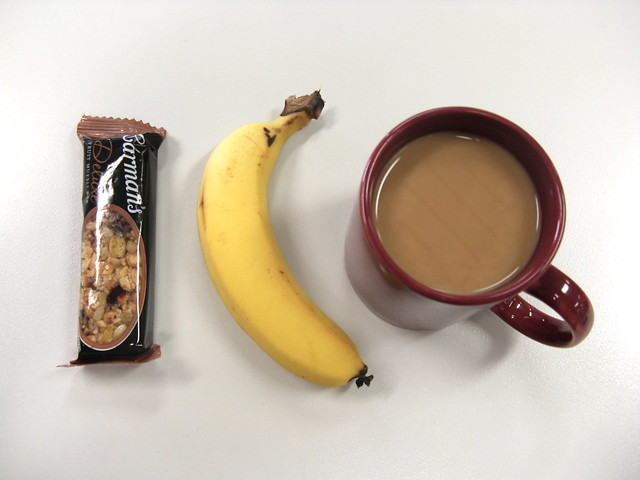
\includegraphics[width=\linewidth, height=2cm]{figs/472228.jpg}
                \vspace{-2mm}
            \end{minipage}
            & 
            \begin{latin}
            \begin{minipage}{.25\textwidth}
                \footnotesize
                \lr{Q: where is a banana?} \\
                \lr{A: a banana sits between a full coffee cup and a granola bar.}
            \end{minipage}  
        \end{latin}
            & 
            \begin{latin}
            \begin{minipage}{.6\textwidth}
                \small
                \lr{LXMERT-3BiLSTM: a banana is on a table with a bowl of scissors.} \\
                \lr{VisualBERT-BahdanauLSTM: a banana sits on a of a a.}\\
                \lr{LXMERT-3Transformer: a banana sits on a table next to a table.}
            \end{minipage}
        \end{latin}
            &
            \begin{minipage} {0.05\textwidth}
            \small        
            WD \\ GE \\ WD
            \end{minipage}
            \\\hline
            \begin{minipage}{.15\textwidth}
                \vspace*{2mm}
                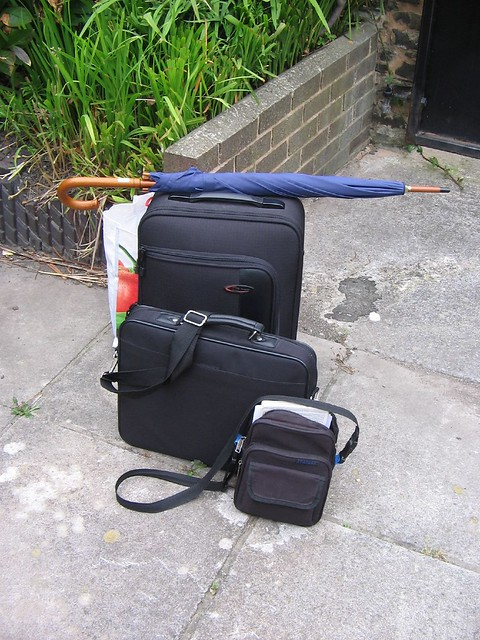
\includegraphics[width=\linewidth, height=2cm]{figs/485799.jpg}
                \vspace{-2mm}
            \end{minipage}
            & 
            \begin{latin}
            \begin{minipage}{.25\textwidth}
                \small
                \lr{Q: what color is the umbrella?} \\
                \lr{A: the umbrella is blue.}
            \end{minipage}  
        \end{latin}
            & 
            \begin{latin}
            \begin{minipage}{.55\textwidth}
                \small
                \lr{LXMERT-3BiLSTM: the umbrella is blue.}\\
                \lr{VisualBERT-BahdanauLSTM: the umbrella is red.}\\
                \lr{LXMERT-3Transformer: the umbrella is blue.}
            \end{minipage} 
        \end{latin}
            &
            \begin{minipage} {0.05\textwidth}
            \small
            EM \\ WA \\ EM
            \end{minipage}   
            \\\hline
             \begin{minipage}{.15\textwidth}
                \vspace*{2mm}
                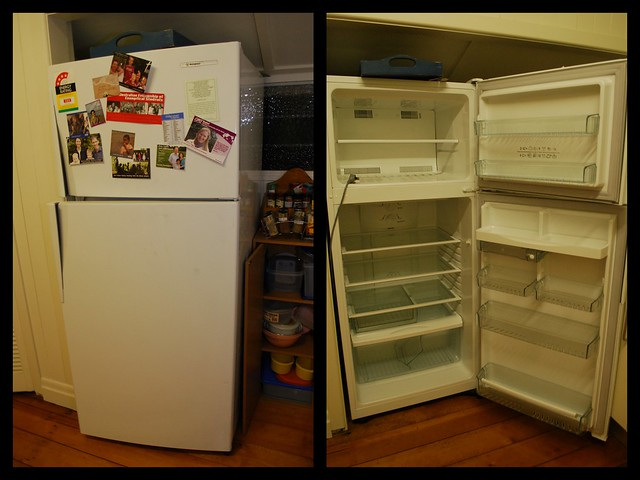
\includegraphics[width=\linewidth, height=2cm]{figs/571585.jpg}
                \vspace{-2mm}
            \end{minipage}
            & 
            \begin{latin}
            \begin{minipage}{.25\textwidth}
                \small
                \lr{Q: what kind of appliance is this?} \\
                \lr{A: this is refrigerator.}
            \end{minipage}  
        \end{latin}
            & 
            \begin{latin}
            \begin{minipage}{.55\textwidth}
                \small
                \lr{LXMERT-3BiLSTM: refrigerator is pictured.} \\
                \lr{VisualBERT-BahdanauLSTM: this is blender.}\\
                \lr{LXMERT-3Transformer: this is refrigerator.}
            \end{minipage}
        \end{latin}
            &
            \begin{minipage} {0.05\textwidth}
            \small
            AA \\ E \\ EM
            \end{minipage}  
            \\ \hline
          \end{tabular}
          }
      \caption{چند نمونه از پاسخ‌ها و اشتباهات آن‌ها بر اساس دسته‌بندی}
      \label{table5}
    \end{table}

    تحلیل این 100 عضو نشان‌داد که تولید پاسخ‌ها باعث کاهش ابهام می‌شود. به عبارت
    دیگر ارائه دادن توضیح اضافه بر کلمه پاسخ باعث می‌شود کاربر از اشتباهاتی
    که سیتم ممکن است منجر بشود را آشکار می‌کند. برای مثال
    فرض کنید پرسش و پاسخ‌های زیر تولید شده باشد:
    \begin{latin}
        \begin{itemize}
            \itemsep-0.3em 
            \item[] \small \lr{\textbf{Question}: Is the dog baring its teeth?}
            \item[] \lr{\textbf{Reference}: No, the dog is not baring its teeth.}
            \item[] \lr{\textbf{Generated}: Yes, the dog is \underline{grillening} its teeth.}
        \end{itemize} 
    \end{latin}
    از آنجایی که کلمه 
    \lr{grillening}
    کلمه‌ای متناسب با حیوانات نیست و حیوانات قادر به انجام آن نیستند، می‌توان از 
    این توضیح اشتباه به درست بودن پاسخ نیز شک کرد. از این رو ارائه توضیح اضافی 
    منجر به رفع ابهامات در پرسش‌وپاسخ تصویری می‌شود. 

    \begin{figure}[H]
        \center{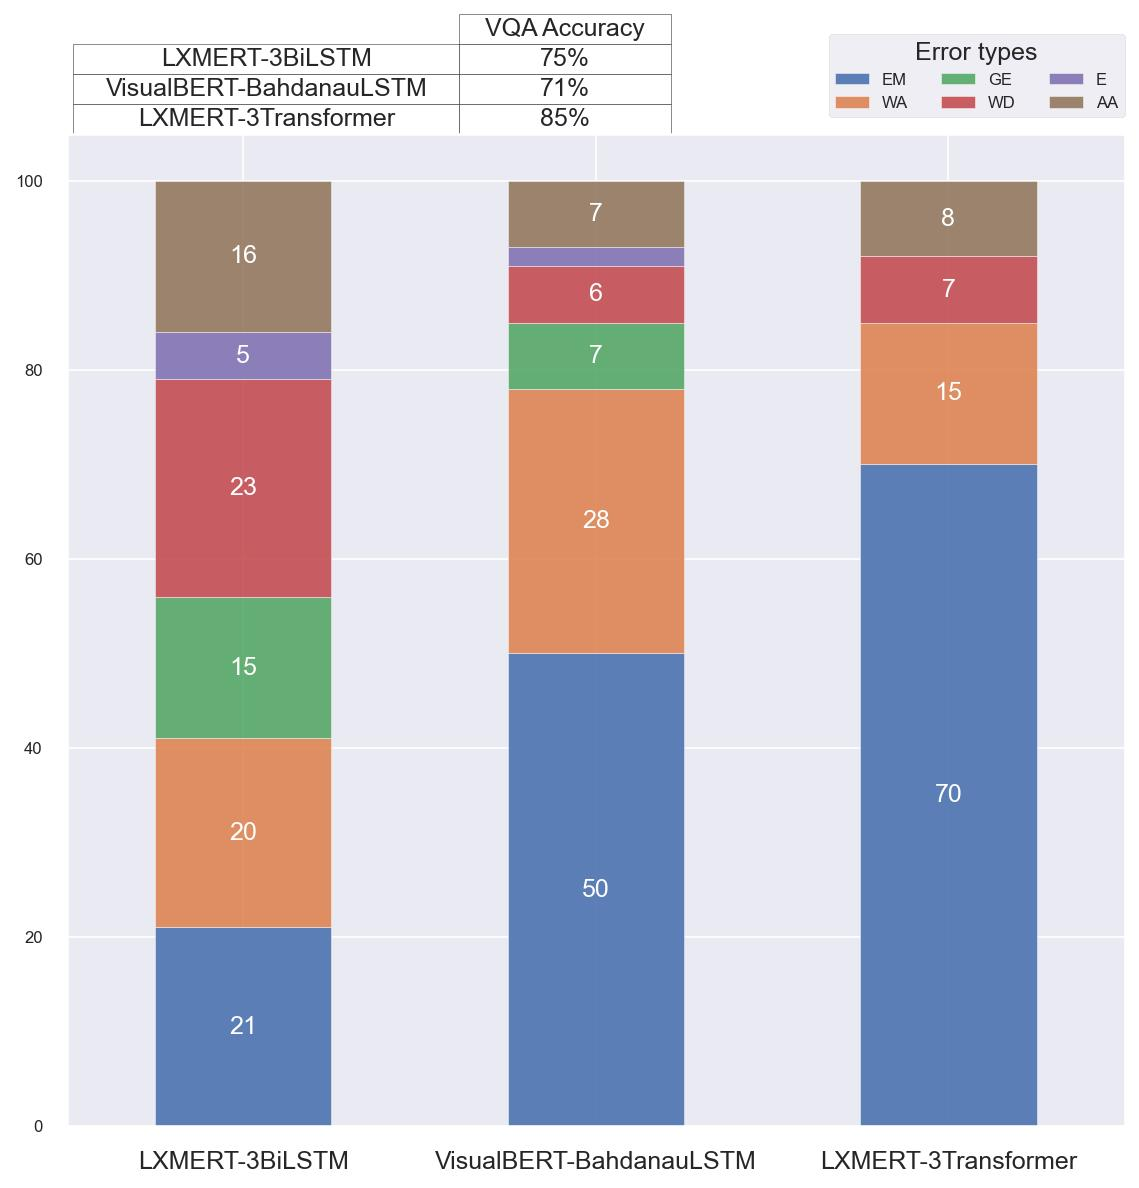
\includegraphics[width=0.7\textwidth]{figs/error.jpg}}
        \caption{نتایج ارزیابی انسانی}
        \label{fig:errors}
    \end{figure}

    شکل 
    \ref{fig:errors}
    نشان‌دهنده عملکرد خوب سیستم را نیز به خوبی نشان می‌دهد، به خصوص اینکه در 
    حالت استفاده مدل‌های تبدیل‌شونده به عنوان کدگشا، هیچ اشتباه گرامری ندارد. 
    یکی دیگر از نتایجی که می‌توان از این تحلیل‌ها گرفت، تاثیر کدگذار است که 
    با توجه به دقت در پرسش‌وپاسخ تصویری، با حضور اشتباهات، همچنان مدلی که 
    LXMERT
    را به عنوان کدگذار استفاده کرده است، دارای دقت بیشتری از 
    مدل‌های بر پایه 
    VisualBERT
    است. 
}
\section{جمع‌بندی}
\paragraph{}
{
    با بررسی نتایج حاصل بر روی مجموعه داده 
    FSVQA
    و سیستم‌های ارائه شده می‌توان نتیجه گرفت استفاده از مدل‌های تبدیل‌شونده 
    به عنوان کدگذار برای تولید پاسخ در پرسش‌وپاسخ تصویری عملکرد بسیار خوبی 
    از خود نشان داده‌است. علاوه بر عملکرد خوب سیتم بر مجموعه داده، با ارزیابی انسانی 
    ثابت شد ارائه دادن توضیح اضافی هنگام پاسخ باعث کمک بیشتر برای فهم پاسخ 
    و حتی در حالاتی منجر به رفع ابهامات می‌شود. با این‌حال هم‌چنان مسیر بسیاری 
    تا حل مسئله پرسش‌وپاسخ تصویری باقی‌مانده است. امتیازات بالایی که در این پژوهش بدست
    آمده‌اند در واقع به علت ساده بودن مجموعه داده است و لازم است
    پرسش‌هایی با پاسخ‌های طبیعی‌تر که از قوانین خاصی پیروی نمی‌کنند موجود
    باشند تا بتوان مقادیر واقعی این معیارها را در محیط‌های واقعی‌تر محاسبه کرد.
}